\documentclass[a4paper,12pt]{article}

\usepackage[utf8x]{inputenc}
\usepackage[english, russian]{babel}

\usepackage{tabularx}
\usepackage{multirow}
\usepackage{graphicx}
\usepackage{longtable}
\usepackage{misccorr}
\usepackage{indentfirst}
\usepackage{amsmath}
%\usepackage{fancynum}


\usepackage{listings}
\usepackage{xcolor}

\usepackage{fullpage}

\usepackage[labelsep=endash,
		    margin=10pt, 
		    justification = centerlast, 
		    format = hang,
		    singlelinecheck=false
		    ]{caption}

\exhyphenpenalty=10000
\doublehyphendemerits=10000
\finalhyphendemerits=5000

\definecolor{codegreen}{rgb}{0,0.6,0}
\definecolor{codegray}{rgb}{0.5,0.5,0.5}
\definecolor{codepurple}{rgb}{0.58,0,0.82}
\definecolor{backcolour}{rgb}{0.95,0.95,0.92}

\newcommand{\tracking}[2]{#2}
\input{letterspacing.tex}\renewcommand{\tracking}[2]{\mbox{\letterspace to #1\naturalwidth{#2}}}
 
\lstdefinestyle{mystyle}{
    backgroundcolor=\color{backcolour},
    commentstyle=\color{codegreen},
    keywordstyle=\color{blue},
    numberstyle=\tiny\color{codegray},
    stringstyle=\color{codepurple},
    basicstyle=\footnotesize,
    breakatwhitespace=false,
    breaklines=true,
    captionpos=t,
    keepspaces=true,
    numbers=left,
    numbersep=10pt,
    showspaces=false,
    showstringspaces=false
    showtabs=false,
    tabsize=4,
    frame=tb
}
 
\lstset{style=mystyle}

\usepackage{color}
\usepackage{xcolor}
\usepackage{listings}
 
% Цвета для кода
 
\definecolor{string}{HTML}{B40000} % цвет строк в коде
\definecolor{comment}{HTML}{008000} % цвет комментариев в коде
\definecolor{keyword}{HTML}{1A00FF} % цвет ключевых слов в коде
\definecolor{morecomment}{HTML}{8000FF} % цвет include и других элементов в коде
\definecolor{сaptiontext}{HTML}{FFFFFF} % цвет текста заголовка в коде
\definecolor{сaptionbk}{HTML}{999999} % цвет фона заголовка в коде
\definecolor{bk}{HTML}{FFFFFF} % цвет фона в коде
\definecolor{frame}{HTML}{999999} % цвет рамки в коде
\definecolor{brackets}{HTML}{B40000} % цвет скобок в коде
 

%%% Отображение кода %%%
 
% Настройки отображения кода
 
\lstset{
	%morekeywords={*,...}, % если хотите добавить ключевые слова, то добавляйте	 
	% Настройки отображения     
	breaklines=false, % Перенос длинных строк
	% Для отображения русского языка
	extendedchars=true,
	literate={Ö}{{\"O}}1
	{Ä}{{\"A}}1
	{Ü}{{\"U}}1
	{ß}{{\ss}}1
	{ü}{{\"u}}1
	{ä}{{\"a}}1
	{ö}{{\"o}}1
	{~}{{\textasciitilde}}1
	{а}{{\selectfont\char224}}1
	{б}{{\selectfont\char225}}1
	{в}{{\selectfont\char226}}1
	{г}{{\selectfont\char227}}1
	{д}{{\selectfont\char228}}1
	{е}{{\selectfont\char229}}1
	{ё}{{\"e}}1
	{ж}{{\selectfont\char230}}1
	{з}{{\selectfont\char231}}1
	{и}{{\selectfont\char232}}1
	{й}{{\selectfont\char233}}1
	{к}{{\selectfont\char234}}1
	{л}{{\selectfont\char235}}1
	{м}{{\selectfont\char236}}1
	{н}{{\selectfont\char237}}1
	{о}{{\selectfont\char238}}1
	{п}{{\selectfont\char239}}1
	{р}{{\selectfont\char240}}1
	{с}{{\selectfont\char241}}1
	{т}{{\selectfont\char242}}1
	{у}{{\selectfont\char243}}1
	{ф}{{\selectfont\char244}}1
	{х}{{\selectfont\char245}}1
	{ц}{{\selectfont\char246}}1
	{ч}{{\selectfont\char247}}1
	{ш}{{\selectfont\char248}}1
	{щ}{{\selectfont\char249}}1
	{ъ}{{\selectfont\char250}}1
	{ы}{{\selectfont\char251}}1
	{ь}{{\selectfont\char252}}1
	{э}{{\selectfont\char253}}1
	{ю}{{\selectfont\char254}}1
	{я}{{\selectfont\char255}}1
	{А}{{\selectfont\char192}}1
	{Б}{{\selectfont\char193}}1
	{В}{{\selectfont\char194}}1
	{Г}{{\selectfont\char195}}1
	{Д}{{\selectfont\char196}}1
	{Е}{{\selectfont\char197}}1
	{Ё}{{\"E}}1
	{Ж}{{\selectfont\char198}}1
	{З}{{\selectfont\char199}}1
	{И}{{\selectfont\char200}}1
	{Й}{{\selectfont\char201}}1
	{К}{{\selectfont\char202}}1
	{Л}{{\selectfont\char203}}1
	{М}{{\selectfont\char204}}1
	{Н}{{\selectfont\char205}}1
	{О}{{\selectfont\char206}}1
	{П}{{\selectfont\char207}}1
	{Р}{{\selectfont\char208}}1
	{С}{{\selectfont\char209}}1
	{Т}{{\selectfont\char210}}1
	{У}{{\selectfont\char211}}1
	{Ф}{{\selectfont\char212}}1
	{Х}{{\selectfont\char213}}1
	{Ц}{{\selectfont\char214}}1
	{Ч}{{\selectfont\char215}}1
	{Ш}{{\selectfont\char216}}1
	{Щ}{{\selectfont\char217}}1
	{Ъ}{{\selectfont\char218}}1
	{Ы}{{\selectfont\char219}}1
	{Ь}{{\selectfont\char220}}1
	{Э}{{\selectfont\char221}}1
	{Ю}{{\selectfont\char222}}1
	{Я}{{\selectfont\char223}}1
	{і}{{\selectfont\char105}}1
	{ї}{{\selectfont\char168}}1
	{є}{{\selectfont\char185}}1
	{ґ}{{\selectfont\char160}}1
	{І}{{\selectfont\char73}}1
	{Ї}{{\selectfont\char136}}1
	{Є}{{\selectfont\char153}}1
	{Ґ}{{\selectfont\char128}}1
	{\{}{{{\color{brackets}\{}}}1 % Цвет скобок {
	{\}}{{{\color{brackets}\}}}}1 % Цвет скобок }
}

\setcounter{tocdepth}{1}

\begin{document}

\begin{titlepage}
\newpage

\

Тут титульник
\end{titlepage}

\newpage
\tableofcontents
\setcounter{page}{2}


\newpage\section{Снижение размерности пространства признаков. Алгоритмы PCA и LDA} 
	Метод главных компонент (principal component analysis, PCA) — один из основных способов уменьшить размерность данных, потеряв наименьшее количество информации. 
	
	\vspace{0.5cm}
	Данный метод аппроксимирует n-размерное облако наблюдений до эллипсоида (тоже n-мерного), полуоси которого и будут являться будущими главными компонентами. И при проекции на такие оси (снижении размерности) сохраняется наибольшее количество информации. 
	
	\vspace{0.5cm}
	Латентное размещение Дирихле (LDA, от англ. Latent Dirichlet allocation) — применяемая в машинном обучении и информационном поиске порождающая модель, позволяющая объяснять результаты наблюдений с помощью неявных групп, благодаря чему возможно выявление причин сходства некоторых частей данных. Например, если наблюдениями являются слова, собранные в документы, утверждается, что каждый документ представляет собой смесь небольшого количества тем и что появление каждого слова связано с одной из тем документа. 
	
	\vspace{0.5cm}
	В LDA каждый документ может рассматриваться как набор различных тематик. Подобный подход схож с вероятностным латентно-семантическим анализом (pLSA) с той разницей, что в LDA предполагается, что распределение тематик имеет в качестве априори распределения Дирихле. На практике в результате получается более корректный набор тематик.

	

\newpage\section{Цель лабораторной работы} 
	Цели: 
	\vspace{0.5cm}
	
	Получить практические навыки по снижению входного пространства признаков
	
	\vspace{0.5cm}
	Задачи: 
	
	\vspace{0.5cm}
	1. Применить к датасету Titanic алгоритм PCA.
	
	\vspace{0.5cm}
	2. Применить к датасету Titanic алгоритм LDA.
	
	\vspace{0.5cm}
	3. Провести ряд экспериментов используя данные из пунктов 1 и 2 и любой из классификаторов, рассмотренных в предыдущих работах.
	
	
\newpage\section{Инструменты} 
	В качестве инструментов для выполнения поставленной цели был выбран язык Python и библиотеки sсikit-learn и Pandas.
	Бибилотека Pandas была использована для подготовки датасета к будущему использованию.
	
	\vspace{0.5cm}
	Для реализации алгоритмов PCA и LDA использовался класс PCA из sklearn.decomposition и класс LinearDiscriminantAnalysis из sklearn.discriminant\_analysis.
	
	\vspace{0.5cm}
	Основные параметры класса PCA.
	
	\vspace{0.5cm}
	n\_components – количество главных компонент.

	
\newpage\section{Эксперименты}
	Для того, чтобы вывести при каких параметрах модель LinearDiscriminantAnalysis и PCA дает наиболее точный прогноз, необходимо провести ряд экспериментов с разными значениями параметров. 
	
	\vspace{0.5cm}
	Для того, чтобы оценить качество уменьшения размерности PCA и качество категоризации LDA,  обучим на полученных данных модель RandomForestClassifier из предыдущей лабораторной работы. Для построения "случайного леса" используем те параметры, при которых в прошлой лабораторной мы получили наилучшие результаты. 
	
	\vspace{0.5cm}
	

	\vspace{0.5cm}
	Таблица 1 - Точность прогнозов  при использовании PCA.
\begin{longtable}{|p{1cm}|p{9cm}|p{3cm}|}
\hline
№ & Параметры & Точность (в процентах) \\ 
\hline 
1 & n\_components=2 & 60.422 \\
\hline
\end{longtable}

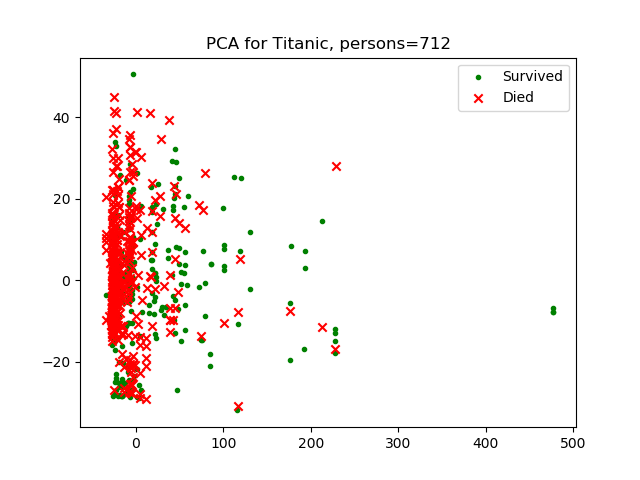
\includegraphics[scale=1]{PCA.png}


\vspace{0.5cm}
	Таблица 2 - Точность прогнозов  при использовании LDA.
\begin{longtable}{|p{1cm}|p{9cm}|p{3cm}|}
\hline
№ & Параметры & Точность (в процентах) \\ 
\hline 
1 & n\_components=2 & 64.652 \\
\hline
\end{longtable}

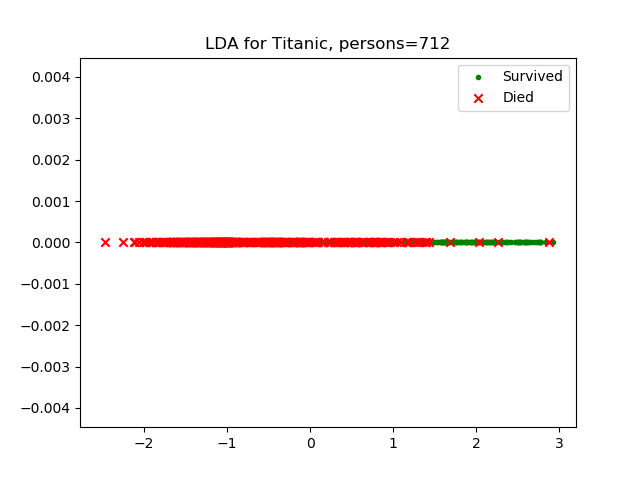
\includegraphics[scale=1]{LDA.png}


\newpage\section{Итог}
	В ходе проведения экпериментов были выявлено, что при изменении данных с помощью алгоритмов PCA и LDA произошло ухудшение результатов работы алгоритма случайного леса. Это может быть связано со структурой набора данных. Так как данные, вероятно, коррелируют между собой, можно предположить, что это сказывается на результатах изменения размерности.
	
	\vspace{0.5cm}
	Также, эксперименты с LDA показали, что параметры модели не оказывают значительного влияния. Поэтому в таблице запечатлен прогноз с параметрами по умолчанию. 
	
	\vspace{0.5cm}
	В случае PCA с параметрами по умолчанию удалось получить наихудший результат. Лучший был получен при параметре svd\_solver равном randomized и большом числе компонент. Исходя из других опытов, можно сделать вывод, что svd\_solver на самом деле не играет большой роли, самым важным параметром является n\_components - размерность выходных данных.
	
	
\end{document}
